\documentclass[11pt,a4paper]{article}

\usepackage[utf8]{inputenc}
\usepackage[spanish,mexico]{babel}

\usepackage{amsmath, amssymb, amsthm}
%\usepackage{mathrsfs}
\usepackage{appendix}
%\usepackage{minted}	

%pdflatex -synctex=1 -interaction=nonstopmode --shell-escape %.tex


\usepackage{hyperref}
\usepackage{captdef}

\usepackage{psfrag}
\usepackage{graphicx}
%\usepackage{subfig}
\usepackage{color}
\usepackage{multicol} 
\usepackage{wrapfig}

%\usepackage{fancyhdr}
%\pagestyle{fancy}
%\fancyhf{}


\usepackage{cancel}
\usepackage[usenames,dvipsnames,svgnames,table]{xcolor}
\usepackage[left=2cm,right=2cm,top=2cm,bottom=2cm]{geometry}
\usepackage{caption}
\usepackage{subcaption}
%\renewcommand{\baselinestretch}{1.5}

\usepackage{hyperref}
%\usepackage[hidelinks]{hyperref} 
\hypersetup{
	colorlinks=true,
	linkcolor=blue,
	filecolor=magenta,      
	urlcolor=cyan,
}

\begin{document}
\thispagestyle{empty}

\includegraphics[height=3.5cm]{escudoCiencias.pdf}
\vspace{-3.8cm}
\begin{flushright}
	\hspace{4cm}
	{\Large\textbf{Sobre los resultados obtenidos}\\
		Proyecto de Tesis}
	\vspace{0.3cm}\\
	\begin{large}Autor: Rodrigo Vega Vilchis.\end{large}\\
	\begin{footnotesize}
		Correo: rockdrigo6@ciencias.unam.mx\\
		\hspace{2.05cm}{\color{white}.}\\
	\end{footnotesize}
	\vspace{0.1cm}
	\begin{large}
		Fecha: 06 Abril, 2024\end{large}\\
\end{flushright}
%\vspace{.4cm}
\hrule height1pt\vspace{.5cm}

\begin{abstract}
	hola
\end{abstract} 
	
\section{Explicaciones técnicas}

El sistema de Lotka-Volterra es uno de los sistemas utilizados para poder comprender la naturaleza de la dinámica no lineal. En este caso particular, los términos no lineales son cuadráticos y representan la interacción entre la especie $i$ y la especie $j$. 
\begin{equation}\label{eqn:LK}
	\frac{dx_i}{dt}=r_ix_i\left(1-\frac{\sum_{j=1}^N \alpha_{ij}x_j}{K_i}\right)
\end{equation}
Se considera una tasa de crecimiento $r_i$ para la especie $i$, una capacidad de carga $K_i$ que limita hasta cierto punto su crecimiento, y su respectiva interacción con la especie $x_j$ cuya ``fuerza'' de interacción esta dada por los coeficientes $\alpha_{ij}$. Al ser un sistema de ecuaciones diferenciales no lineales, no es posible acceder a una solución analítica general\footnote{debido a los términos no lineales... (me gustaría una explicación más completa: ver strogatz y tratados de ecuaciones diferenciales).}; por ello se recurre a métodos de integración numérica capaces de aproximar las soluciones a un rango considerable y cercano a la solución real. El método empleado por excelencia en este trabajo es el integrador Runge-Kutta de orden 4\footnote{poner una referencia de libro}.\\
\\
De manera pedagógica para aprender y analizar las virtudes y comportamientos del sistema \ref{eqn:LK} es recomendable comenzar por explorar el sistema de $2\times 2$.
$$
\begin{cases}
	\dot{x}_1&=r_1x_1(1-\frac{a_{11}x_1}{k_1}-\frac{a_{12}x_1x_2}{k_1})\\
	\dot{x}_2&=r_2x_2(1-\frac{a_{21}x_1x_2}{k_2}-\frac{a_{22}x_2}{k_2})
\end{cases}
$$
En este caso particular, tenemos una tasa de crecimiento y una capacidad de carga personalizada para cada especie, lo que es razonable con el hecho de que cada especie crece a un ritmo determinado y también es limitada de manera determinada. En este caso los coeficientes $\alpha_{ij}$ forman parte de una matriz de \textit{incidencias} entre especies definida de la siguiente manera
$$A=
\begin{pmatrix}
	1 & \alpha_{12}\\
	\alpha_{21} &1
\end{pmatrix}
$$
Es apreciable que los términos de la diagonal se encuentran en $\alpha_{ii} = 1$\footnote{Argumentar más adelante.} respectivamente, más adelante se dará una explicación detallada de esta característica; por el momento solo nos enfocaremos en la dinámica que produce el sistema. Para ello se define el siguiente sistema
\begin{align*}
	\frac{dx}{dt}&=2x\left(1-\frac{x}{2}\right)-xy\\
	\frac{dy}{dt}&=3y\left(1-\frac{y}{3}\right)-2xy
\end{align*}
De este sistema se pueden notar algunas características: se tiene para cada ecuación diferencial (especie) una tasa de crecimiento y una capacidad de carga específica o personalizada. Por ejemplo para la ecuación $\dot{x}$ se tiene una tasa de crecimiento y capacidad de carga de 2 para la especie $x$ y para la especie $y$ estos valores son iguales a 1; para la ecuación $\dot{y}$ se tiene una tasa de crecimiento y capacidad de carga de 3 para la especie $x$ y para la especie $y$ se tiene una tasa de crecimiento de 2 y una capacidad de carga de 1. Aunque este sistema tal cual no tiene una solución analítica per se, si es posible explorar acerca de su comportamiento; en principio se pueden hallar sus puntos fijos que nos hablan de la estabilidad del sistema. Para hallar puntos fijos es necesario encontrar las raíces de este sistema. La solución trivial siempre será $(0,0)$, de ahí se tienen que igualar a cero las ecuaciones para hallar los otros puntos críticos.
\begin{align*}
	2x-x^2-xy &= 0,\qquad\text{suponiendo que $y = 0$}\\
	2x &= x^2\\
	x&=2
\end{align*}
y para $\dot{y}$ se tiene
\begin{align*}
	3y-y^2-2xy&=0,\qquad\text{suponiendo que $x=0$}\\
	3y &= y^2\\
	y &= 3
\end{align*}
Por tanto tenemos para $\dot{x}$ el punto fijo $(2,0)$ mientras que para $\dot{y}$ se tiene el punto fijo $(0,3)$. Aún es posible hallar un último punto fijo que es para cuando ambas ecuaciones se hacen cero.
\begin{align*}
	2x-x^2-xy&=0,\qquad\text{Se despeja $y$ de esta ecuación.}\\
	xy &= x(2-x)\\
	y &= (2-x)\\
	\\
	3(x-2)-(x-2)^2-2x(x-2) &= 0\\
	3x-6-(x^2-4x+4)-2x^2+4x&=0,\qquad\text{Reduciendo términos se tiene.}\\
	x^2-3x+2 &= 0
\end{align*}
%%%%%%%%%%%%%%%%%%%%%CHECKPOINT
Al resolver esta última ecuación se determina el último punto fijo que corresponde a $(1,1)$. Los puntos fijos brindan información para explorar hacia donde pueden converger (atractores) o diverger (repulsores o puntos sillas) las soluciones del sistema dependiendo de las condiciones iniciales que se le impongan.\footnote{explicar brevemente de que se trata uno, quizás esto deba precisarse desde la introducción.} Se establece que si las soluciones convergen entonces el sistema es considerado \textit{estable} mientras que 
\begin{wrapfigure}{r}{0.5 \textwidth} \vspace{-30pt} \begin{center}
		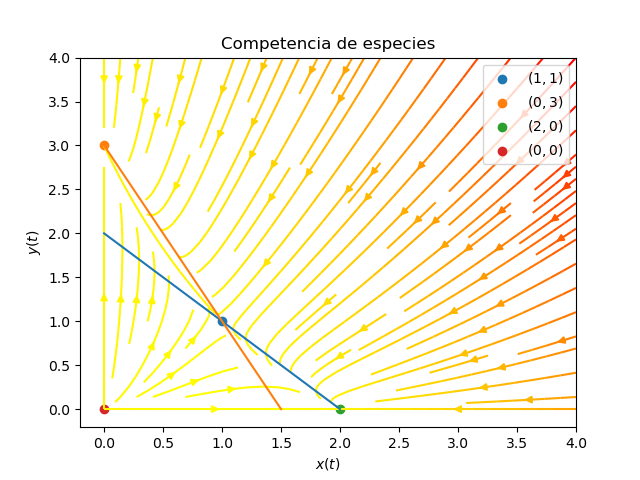
\includegraphics[width=0.45\textwidth]{Competencia de especies} 
		\end{center} 
		\vspace{-20pt} 
		\caption{Campo vectorial de las soluciones del sistema propuesto.} 
		\vspace{-10pt}
		\label{fig:CompetenciaEspecies}
\end{wrapfigure} 
en caso contrario el sistema es considerado \textit{inestable.} Es posible determinar mediante técnicas computacionales el campo vectorial de las soluciones de este sistema\footnote{Realizar referencia de la técnica empleada.}, inclusive dos de las isoclinas\footnote{si son isoclinas???} del sistema resolviendo las ecuaciones igualando a cero y despejando $y$ de cada una de ellas. Es notorio como dichas isoclinas inciden de alguna forma en tres de los puntos fijos. El gráfico nos muestra que las soluciones convergen hacia los puntos que se encuentran en los ejes; todo dependerá de las condiciones iniciales del sistema para ver hacia donde convergen. El punto fijo de en medio es conocido como punto silla y es inestable ya que aunque existan soluciones que convergan hacia él mismo, en la mínima perturbación que se le provoque la solución puede ``desviarse'' hacia los atractores. Por último se observa que del origen divergen todas las soluciones por lo que es considerado un punto fijo repulsor.\\
\\
En esta ocasión por tratarse de un sistema de $2\times 2$, se tuvo la fortuna de poder obtener una representación visual del sistema y poder realizar un análisis cualitativo del mismo para sacar conclusiones. Pero ¿qué sucede cuando se tienen sistemas de $N$ especies? En principio el espacio vectorial (fase) de las soluciones se vuelve $N-$dimensional y por lo tanto imposible de visualizar en un gráfico. Es por ello que se requieren de otras técnicas analíticas para seguir esbozando el comportamiento del sistema. Una herramienta útil a esta conjetura es la de \textit{linealizar} el sistema para poder explorar el comportamiento de los puntos fijos a nivel local. Para realizar esta acción es necesario aplicar el Jacobiano al sistema para ``bajar'' el grado de las ecuaciones a ecuaciones no lineales del sistema.\\
\\
Definiendo al sistema de la siguiente manera
\begin{equation}\label{eqn:LKmatricial}
	\mathbf{F}(t)=\begin{pmatrix}
		\dot{x}_1\\
		\vdots\\
		\dot{x}_n
	\end{pmatrix}
\end{equation}
donde el vector de derivadas temporales de \ref{eqn:LKmatricial} corresponden con el sistema generalizado de Lotka-Volterra \ref{eqn:LK}. Entonces el jacobiano es esta función vectorial se vería de la siguiente forma
\begin{equation}
	\mathbb{J}(\mathbf{F}) = \begin{pmatrix}
		
	\end{pmatrix}
\end{equation}


\end{document}